Um die oben genannten Spiele um einen virtuellen Teil erweitern zu k�nnen werden Konzepte ben�tigt. Eine von uns getroffene Auswahl wird im folgenden beschrieben. 

\section{Erweiterte Realit�t}
Konzepte, die explizit die Realit�t erweitern und somit einen Mehrwert zum Spiel beitragen.


\subsubsection{Integration virtueller Objekte in die physische Umgebung}
Um ein virtuelles Spiel in die physische Umgebung integrieren zu k�nnen, m�ssen auch alle Objekte
des virtuelles Spieles in die physische Umgebung gebracht werden.
Bei vielen Objekten kann dies durch einen eingeschr�nkten Zufall geschehen. Z.B. bei Snake die 
Items. Bei dem ein oder anderen Spiel soll es eine Basis f�r jedes Team geben. Dabei bietet sich an
dieses auf eine relativ freie Fl�che festzusetzen. Generell sollte darauf geachtet werden, 
dass die Objekte nicht innerhalb eines Geb�udes landen oder in nicht begehbares Terrain platziert werden.



Dies kann mit Hilfe der folgenden technischen L�sungen umgesetzt werden:
Kartendarstellung (s. \ref{kartendarstellung}), Kollisionsabfrage (s. \ref{kollisionsabfrage}), Positionsabfrage (um sicherzustellen, dass das Objekt in der N�he des Spieler erstellt wird, s. \ref{positionsermittlung}).

\subsubsection{Darstellung der physischen und virtuellen Umgebung}

Die physische Welt in eine virtuelle Umgebung zu �bertragen kann oft sehr hilfreich sein.
Sei es in einer Karte als �bersicht oder lediglich eine Anzeige ob man sich innerhalb bzw.
au�erhalb des Spielfelds befindet. 
\begin{figure}[htbp]
  \centering
    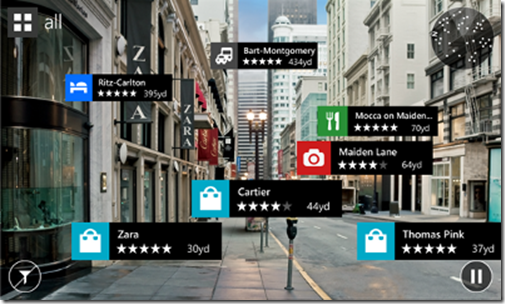
\includegraphics[width=0.9\textwidth]{3-Spielkonzepte/3-1-Erweiterte_Realitaet/map01.png}
     \caption{Handyscreen um die zu sehenden Gesch�fte, Hotels, etc. erweitert}
\end{figure}
 Eine Karte hat insoweit den Vorteil, dass man dort auch
noch virtuelle Gegenst�nde einf�gen kann, die in der physischen Welt nicht vorhanden
sind. Z.B. die n�chsten Items bei Snake.
Dazu sind 
Kartendarstellung (s. \ref{kartendarstellung}) und Positionsermittlung (s. \ref{positionsermittlung}) n�tig.

\subsubsection{Kollision virtueller Objekte}
Treffen zwei virtuelle Objekte aufeinander muss in der Regel ein Event ausgel�st werden.
Wird bei Snake z.B. der eigene Schwanz ber�hrt, was laut der Regeln nicht erlaubt ist, muss
dies dem Spieler mitgeteilt werden und evtl. weitere Ereignisse ausgef�hrt werden.
\newline
Technische L�sungen:
Kollisionsabfrage (s. \ref{kollisionsabfrage}), Positionsermittlung (s. \ref{positionsermittlung})


\subsubsection{Einsammeln von Objekten}
Eine Variante der Kollision mit virtuellen Objekten ist das Einsammeln. Wenn ein Spieler in
Reichweite eines Items ist, das es einzusammeln gilt, kann dies entweder automatisch
passieren oder �ber eine Aufforderung auf dem mobilen Ger�t. Zur Best�tigung, dass
etwas eingesammelt wurde, kann nun wiederum ein akustisches oder haptisches Signal
gegeben werden.


Technische L�sungen:
Positionsermittlung (s. \ref{positionsermittlung}), Kollisionsabfrage (s. \ref{kollisionsabfrage})